% --- Ejercicio 1 -------- %
\begin{ejercicio}
    Calcular la magnitud, argumento, parte real y parte imaginaria de los siguientes números complejos:
    %
    \begin{enumerate}
        \item $(1+j\sqrt{3})^{1+i}$
        \item $\sqrt{-j}$
    \end{enumerate}
\end{ejercicio}

% --- Ejercicio 2 -------- %
\begin{ejercicio}
    Sean $z$, $w \in \mathbb{C}$. Se sabe que $z=\frac{3}{2}+j$, $\textit{Re}\{w\} = \frac{1}{2}$ y $|z+w|=3$. Encuentre gráficamente $w$ y $z+w$.
\end{ejercicio}

% --- Ejercicio 3 -------- %
\begin{ejercicio}
    Dadas las siguientes condiciones geométricas, hallar $z \in \mathbb{C}$:
    \begin{itemize}
        \item $|j+z^*| = 5$
        \item $\angle(z+2) = -\frac{3\pi}{4}$
    \end{itemize}
\end{ejercicio}

% --- Ejercicio 4 -------- %
\begin{ejercicio}
    Determinar las cinco raíces de $(-1)^{1/5}$.
\end{ejercicio}

% --- Ejercicio 5 -------- %
\begin{ejercicio}
    Calcular las soluciones de la ecuación $z^4+(1+j)z^2+5j=0$.
\end{ejercicio}

% --- Ejercicio 6 -------- %
\begin{ejercicio}
    El circuito de la figura \ref{fig:circuito} se utiliza para calcular el valor de $R_C$, la cual modela las pérdidas en el dieléctrico del condensador.\par
    Con un voltímetro digital, se ha determinado que la tensión RMS en la fuente es $V_S=1$V, la tensión RMS en la resistencia de medición $R_m$ es $V_{R_m}=0.3$V y la tensión RMS en el condensador real (la región demarcada) es $V_c=0.8$V.\par
    Determine gráficamente cuál es el valor de $C$ y $R_C$ si se sabe que la fuente utiliza una frecuencia de $100$Hz y $R_m = 1$M$\Omega$.
    \label{ejercicio_circuito}
    \begin{figure}
        \centering
        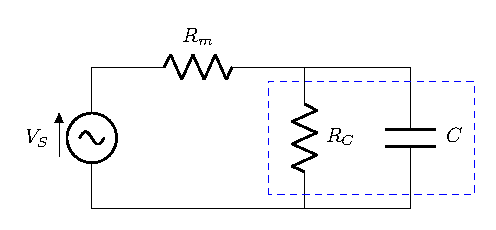
\includegraphics[width=0.6\linewidth]{figs/circuit.pdf}
        \caption{Circuito de referencia del ejericio \ref{ejercicio_circuito}.}
        \label{fig:circuito}
    \end{figure}
\end{ejercicio}

% --- Ejercicio 7 -------- %
\begin{ejercicio}
    Encuentre las ecuaciones de las siguientes rectas en el plano $z$ para la forma cartesiana $y=mx+b$:
    \begin{enumerate}
        \item $|z-2+j| = |z-j+3|$
        \item $|z+z^*+4j(z-z^*)| = 6$
    \end{enumerate}
\end{ejercicio}

% --- Ejercicio 8 -------- %
\begin{ejercicio}
    Encuentre el punto de intersección y el ángulo de intersección de las rectas:
    \begin{itemize}
        \item $|z-1-j|=|z-3+j|$
        \item $|z-1+j|=|z-3-j|$
    \end{itemize}
\end{ejercicio}

% --- Ejercicio 9 -------- %
\begin{ejercicio}
    Indique qué mapeos elementales (rotación, escalado y traslación) realiza el siguiente mapeo:
    $$ w = (\sqrt{3}+j)z - j $$
\end{ejercicio}
